\scanpage{233}
ce complexe est déduit d'une résolution flasque $\widetilde\Phi_*^{p*}$ de
\deleted{$\unsure{\Phi}$} $k_*$ en le ``tronquant'' en \deleted{dim} degré $\leq p$,
i.e. en prenant $\Phi_*^{p*}=\tau^{\leq p}\widetilde\Phi_*^{p\unsure{*|2}}$
\margin{\deleted{$\unsure{\Phi}$}}
\[
\Phi_*^{pi}=\begin{cases}
\widetilde\Phi_*^{p,i}&\text{si }i<p\\
Z^p(\widetilde\Phi_*^{p,*})&\text{si }i=p\\
0&\deleted{\text{à}}\text{ si }i>p
\end{cases}
\]
Par suite, pour tt $X$ semi-simplicial, on aura
\[
\begin{aligned}
\underset{\substack{\Vert\,\mathrm{déf}\\C_{\mathrm{DRpd}}^{p*}(X,k)}}{\operatorname{Hom}(X,\Phi_*^{p*})}
&\simeq\deleted{\unsure{\Gamma}}\unsure{\operatorname{Hom}|\Gamma}
(X,\tau^{\leq\unsure{p|n}}\widetilde\Phi_*^{p*})
\simeq\tau^{\leq p}\Gamma(X,\widetilde\Phi_*^{p*})\\
&\simeq\tau^{\leq p}\mathbb R\Gamma(X,k).
\end{aligned}
\]
En particulier
\[
H_{\mathrm{DRpd}}^{p*}(X,k)\mathbin{-}H^*(X,k)
\]
\deleted{est un isom} tel que
\[
H_{\mathrm{DRpd}}^{pi}(X,k)
\left\{\begin{aligned}&\xrightarrow{\sim}H^i(X,k)&&\text{si }i\leq p\\
&=0&&\text{si }i>p.
\end{aligned}\right.
\]
\figure{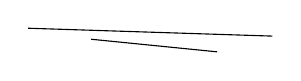
\begin{tikzpicture}[x=1cm,y=1cm]
\draw (0,0)--(3.1,-.10);\draw (.8,-.14)--(2.4,-.30);
\end{tikzpicture}}

Soit $S$ anneau avec idéal $S^+$ à p.d., muni d'un
\deleted{\unsure{suite décroissante}} $t\in S^+$.
Quitte à remplacer $S$ par son séparé complété pour la top. engendrée par les idéaux
\[
S^{[i]}=\text{idéal engendré par les }t^{(j)}\quad(j\geq i)
\]
on se suppose $S$ séparé et complet pour la top définie par une suite décroissante
d'idéaux $S^{[i]}$, chacun dans l'adhérence de l'idéal engendré par $t^{(j)}$ $(j\geq i)$.
\margin{232}
